\subsection*{a)}

\begin{equation}
\label{eq:partSt}
\frac{\partial S}{\partial t} = b(S+I)-cS -\frac{S(I+S)}{K}-aSI + D\nabla^2S,
\end{equation}

\begin{equation}
\label{eq:partIt}
\frac{\partial I}{\partial t}= -cI -\frac{I(I+S)}{K}+aSI +D\nabla^2I.
\end{equation}

For the spatially homogeneous model, that is $D=0$ we have the steady states when

$$
\frac{\partial S^*}{\partial t}=b(S^*+I^*)-cS^*-\frac{S^*(I^*+S^*)}{K}-aS^*I^* =0
$$

and

$$
\frac{\partial I^*}{\partial t}=-cI^*-\frac{I^*(I^*+S^*)}{K}+aS^*I^*=0.
$$

We can directly rule our the steady states which involve $S^*\leq0$ or $I^*<0$.

\begin{itemize}
\item $S^*_1=K(c-b), \;\; I^*_1=0$
\item $S^*_2=\frac{b}{a}, \;\; I^*_2=K(b-c)-\frac{b}{a}$ 
\end{itemize}



To see the stability of these steady states we need to consider the jacobian for theses states,

\begin{equation}
\mathbb{J}^*_n=\left.\left(
\begin{array}{cc}
\frac{\partial f}{\partial S} & \frac{\partial f}{\partial I} \\
\frac{\partial g}{\partial S} & \frac{\partial g}{\partial I}
\end{array}\right)\right|_{(S^*_n,I^*_n)},
\end{equation}

where 

\begin{equation}
f(S,I)=b(S+I)-cS-\frac{S(I+S)}{K}-aSI
\end{equation}

\begin{equation}
g(S,I)=-cI-\frac{I(I+S)}{K}+aSI.
\end{equation}

So
\begin{equation}
\mathbb{J}^*_n=\left.\left(
\begin{array}{cc}
b-c-\frac{I+2S}{K}-aI & b-\frac{S}{K}-aS \\
-\frac{I}{K} +aI & -c -\frac{2I+S}{K}+aS
\end{array}\right)\right|_{(S^*_n,I^*_n)},
\end{equation}

To have a stable steady state we need that 

\begin{enumerate}
\item $Tr(\mathbb{J}^*_n)<0$
\item $Det(\mathbb{J}^*_n)>0$
\end{enumerate}


For the first steady state we get that the steady state is stable for

$$
K>\frac{3c}{a(c-b)}
$$$$
K<\frac{2c-b}{a(c-b)}
$$

which can't be fulfilled at the same time.

For the second steady state however the conditions given above don't contradict each other and we can find $K_c$ as follows

\begin{equation}
K_c=Max\left[\frac{b}{a(b-c)},\frac{2b-3c}{a(b-c)}\right]
\end{equation}

\subsection*{b)}

The introduction of the new variable $N=I+S$, which is the total population, inserted into equations \eqref{eq:partIt} and \eqref{eq:partSt} gives,

\begin{equation}
\frac{\partial N}{\partial t}=bN -cN -\frac{N^2}{K}+D\nabla^2N.
\end{equation}

If we assume that we are studying the dynamics in one dimension, we can replace the $\nabla^2$ operator with a second derivative in that direction, i.e. $\nabla^2\rightarrow \frac{\partial^2}{\partial x^2}$ and we get the time evolution as,

\begin{equation}
\frac{\partial N}{\partial t}=(b-c)N\left(1-\frac{N}{K}\right)+D\frac{\partial^2 N}{\partial x^2}.
\end{equation}

To see if the dynamics exhibits a travelling wave solution we try to reduce the spatial and temporal dimension to one by $z=x-ct$, and changing the population variable to $N(x,t)\rightarrow u(z)$ which would yield,

\begin{equation}
-c\frac{\partial u}{\partial z}=(b-c)u\left(1-\frac{u}{K}\right)+D\frac{\partial^2 u}{\partial x^2}.
\end{equation}

To study the dynamics of this system introduce yet another variable, $v=\frac{\partial u}{\partial z}$, and receive the system 

\begin{align*}
\frac{\partial u}{\partial z}&=v\\
\frac{\partial v}{\partial z}&=-\frac{c}{D}v-\frac{(b-c)u(1-\frac{u}{K})}{D}.
\end{align*}

This system has the steady states $(u^*,v^*)=(0,0)$ and $(u^*,v^*)=(K,0)$.

To check the stability of these steady states we need to consult the Jacobian matrix,

\begin{equation}
\mathbb{J}=\left(\begin{array}{cc}
0 & 1 \\
  \frac{(b-c)(K-2u)}{KD} & -\frac{c}{D}
\end{array}\right),
\end{equation}

 evaluated at the steady states. To check the stability of the steady states we need to check the signs of the determinant and trace of the jacobian, and the value of the determinant for these states are,
 
 $$
 det(\mathbb{J}^*_1)= -\frac{b-c}{D}<0
 $$
 and
 
 $$
 det(\mathbb{J}^*_2)=\frac{b-c}{D}>0.
 $$
 
 Their traces does not depend on the steady state itself and they are therefore the same 
 $$
 Tr(\mathbb{J}^*_1)=Tr(\mathbb{J}^*_2)=-\frac{c}{D}<0.
 $$
 
The first state has $det(\mathbb{J}^*)<0$ and $Tr(\mathbb{J}^*)<0$ which makes it a candidate for being both a saddle point and a stable spiral. It is a saddle point if $c^2_s>4D(b-c)$ and a steady spiral if $c^2_s<4D(b-c)$. To get a travelling wave solution we need to go from the steady state with a low amount of population, i.e. the first steady state, to the second one. To accomplish this we need the first steady state to be a saddle point, otherwise there is no way for the population to increase.\\
So now we have an expression for the velocity $c_s$ when we have a saddle point and the minimum velocity is thusly,

$$
 c^2_s>4D(b-c)\Rightarrow c_s > \sqrt{4D(b-c)}.
 $$
 
\subsection*{c)}

\begin{figure}
\centering
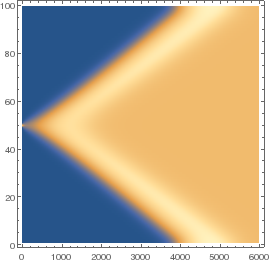
\includegraphics[scale=0.5]{img/listdensityplot_S.png}
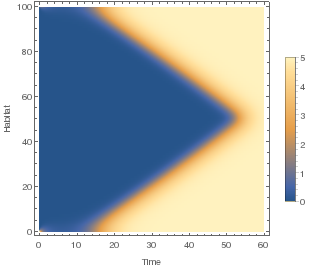
\includegraphics[scale=0.5]{img/listdensityplot_P.png}
\caption{\label{fig:pic1c} In the left panel, depicting the development of the suseptible individuals $S$ in time and space, we can calculate the speed of the seen traveling wave by $c=\frac{\delta x}{\delta t}$. The same can be done for the infected individuals $I$ in the right panel.}
\end{figure}

We can see the expansion of the susceptibles $s$ in the left panel of figure \ref{fig:pic1c}. The population expands in both directions with equal constant velocity and expansion resembles a traveling wave. The steady state for the spatially inhomogeneous suceptible habitat size are the same as the homogeneous steady stable state which is $10$. The speed of this traveling wave is estimated to $1.35$. We see in the figure that the number of susceptibles overshoots over the steady state, which might suggest that the   Carrying capacity term of the system is delayed which is actually seen in the right panel where the number of infected to rise after some time delay. \\

We see that the number of infected does not overshoot, but stops at the steady steate $I^*=5$. We can also calculate the velocity to $1.33$ which is just below the velocity for the susceptibles. This might be because the number of infected depends on the number of susceptibles of the previous batch and have a harder time to catch up to the number of susceptibles.
